\documentclass[conference,compsoc]{IEEEtran}
\usepackage{graphicx, subcaption}
\usepackage{algorithm, algpseudocode}
\usepackage{enumitem}
\usepackage{fixltx2e}
\usepackage{booktabs}
\usepackage{amssymb}
\hyphenation{op-tical net-works semi-conduc-tor}


\begin{document}
\title{Cache-aware data structures for packet forwarding tables on general purpose CPUs}
\author{\IEEEauthorblockN{Maksim Yegorov}
\IEEEauthorblockA{Computer Science Department\\
Rochester Institute of Technology, NY\\ Email: \texttt{mey5634@rit.edu}
}}

\maketitle

\begin{abstract}
TBD...

\end{abstract}

\section{Background}
To set the context, consider the fundamental task of a network router.
In order to match an incoming packet to an outgoing interface link,
the router inspects the packet's header to obtain the destination address.
It will then consult a forwarding (Forwarding Information Base) table 
stored on the router.
An address entry in such a table will contain, among other things,
a variable length prefix (as in 129.12.30.0/20).
In effect, the router will compare the destination IP
against the known prefixes using the longest prefix match rule.
The forwarding table itself may be occasionally updated with new prefixes
received via BGP route advertisement \cite{Kurose:Networking}.

It would appear that a standard hash table or a binary search tree could
satisfy the requirements of a data structure that permits the 
\textit{look-up} and \textit{update} operations. The difficulty with 
adapting the well-known 
datastructures for Internet routing stems mainly from the sheer throughput
demand imposed by today's line speed and the FIB table size.
This can be easily shown on the example of a hypothetical 50Gbps core router 
and an Ethernet frame of 84 bytes for a minimum sized packet. 
The bit per second 
wire line speed can be framed in terms of packets per second. Specifically,
for this simplified scenario, we can expect to process 75Mpps. Depending on
the algorithm that we pick, this may require at least 75 million lookups 
per second (or an order of magnitude more). For a general purpose CPU clock
speed of (for the sake of example) 4 GHz, this equates to approximately 
50 CPU cycles per packet. If the router cannot keep up with the speed of
arriving packets, it will drop packets.

How much work can be done in 50 CPU cycles? As a very rough approximation,
consider that conventional hashing algorithms require about 10 cycles 
per byte of hash (40 cycles to compute a 32 bit hash). Memory latency
presents a particular challenge. The access times range between 4-50 cycles
for L1 and L3 CPU caches, respectively. The penalty for misses can easily 
double the time requirements. Main memory access will require several hundred 
cycles.

Clearly, this hypothetical scenario is an oversimplication. The forwarding
task is only one among many processing steps that a router performs on each
packet, contemporary CPUs will likely have multiple cores, router line
speeds may be in the single digits or in the hundreds of Gbps, there will 
be a distribution of packet sizes (my estimate errs on the conservative
side), leaf node routers may benefit from caching previously seen IP
addresses etc. Still, the above generalization gives us a ballpark number 
to quickly determine if a particular datastructure is fit for the task.

In view of these numbers, it is not at all surprising that the lookup has 
been traditionally performed in hardware, using dedicated TCAM and SRAM 
circuits. There are multiple considerations that make software 
implementations superior to ASIC hardware based ones. The cost per 
transistor, power requirements, and monopoly effects, in particular, 
drive up the cost. The inability to patch hardware makes security updates
unfeasible. There has been a renewed push recently to develop 
programmable routers that, on the one hand, can accommodate the data 
processing speeds expected of today's networks, and on the other, offer 
the option to implement and continuously update various parts of the 
network stack in software rather than hardware.


\section{Related Work}
Classical algorithms developed up to about 2007 have been surveyed in
\cite{Sanchez:Survey} and \cite{Varghese:Algorithmics}. 
The data structures include trie, tree, and hash table variants.

Of particular relevance is the binary search on prefix lengths
proposed in \cite{Waldvogel:Scalable}. Waldvogel et al. propose a very 
elaborate hash table of binary search trees with logarithmic time 
complexity. Most
of the refinements involve comparatively large databases that require at
least an order of magnitude more memory than what can fit into third level
cache, and are therefore only practical for hardware implementations. We
believe that the core ideas of leveraging the binary search on prefixes and 
using memoization to avoid backtracking when the search fails can be
adapted to the more compact data structures.

Dharmapurikar et al.\cite{Dharmapurikar:Bloom} describe a longest prefix
matching algorithm utilizing a probabilistic set membership check with
Bloom filters. A Bloom filter is associated with each prefix length. The
destination adress is masked and matched against each of the Bloom filters,
yielding a list of one or more prefix matches. The list is then checked
against an off-chip conventional hash table, starting with the longest 
prefix match. Because of the arbitrarily small false positive rate, 
a single lookup in high-latency main memory is sufficient in practice.

\section{Solution}

\subsection{Goals}

We have identified two opportunities for improvement in the context of
the Bloom filter-based solutions to the longest prefix matching problem.
The Bloom filter (BF) data structure was originally used by 
Dharmapurikar et al. \cite{Dharmapurikar:Bloom}
for parallel look up implemented in hardware. By contrast, the software
implementations on conventional hardware pay a hefty penalty -- in computation
cost and code complexity -- to parallelize the look up. The default solution
has been a linear search (see Algorithm~\ref{alg:linearsearch}). The time
complexity of Algorithm~\ref{alg:linearsearch} is $\mathcal{O}(n)$, where $n$
is the number of distinct prefix lengths in the BF. We
propose to improve on the linear search for Bloom filter in this paper.

\begin{algorithm}
\caption{Linear search for longest matching prefix}\label{alg:linearsearch}
\begin{algorithmic}[1]
\Procedure{LinearSearch}{$bf, ip, fib, maxlen$}
\State $plen \gets maxlen$\Comment{max prefix length}
\While{$plen \geq \textsc{minlen}$}\Comment{min prefix length}

  \State $tmp \gets$ extract $plen$ most significant bits in IP
  \State $key \gets \texttt{encode(tmp, plen)}$
  \State $res \gets \texttt{bf.contains(key,}$
                \State $\hspace*{36mm} \texttt{[hash\textsubscript{1}..hash\textsubscript{bf.k}])}$
  \If{$res \not= 0 \;\&\; key \in fib$}
      \State \textbf{return} $plen$
  \Else
    $\;plen \gets plen - 1$
  \EndIf
\EndWhile
\State \textbf{return} \textsc{pref\textsubscript{default}}\Comment{default route}
\EndProcedure
\end{algorithmic}
\end{algorithm}


Second, any scheme that utilizes a probabilistic data structure, such as
the Bloom filter, to identify candidate(s) for the \emph{longest matching
prefix} (LMP) would generally need to look up the candidate(s)
in a forwarding table that serves as the definitive membership
test and the store of the next hop information. Current solutions typically
store this information in an off-chip hash table. This operation is therefore
a bottleneck of the probabilistic filter-based schemes. While we have
not yet implemented or tested the proposed guided search data structure
specifically for FIB storage, we conjecture that the method we propose may be broadly
applicable to any key-value store application that

\begin{enumerate}[label=(\alph*)]
\item is defined as a many-to-few kind of mapping over totally ordered keys, and
\item tolerates (i.e. self-corrects for) a certain probability of error.
\end{enumerate}

In the case of the FIB table, we propose to store the outgoing link information
in a compact array. We would then insert encoded \texttt{(index, prefix)} pairs
into a \emph{guided BF} data structure (separate from the BF used to
encode \texttt{(length, prefix)} pairs). For forwarding table applications, this appears 
feasible on today's off-the-shelf hardware, where we would typically have 
on the order of a
million keys, with array indices (outgoing interfaces) numbering in the low 
hundreds.

From our preliminary analysis, both Bloom filters (\texttt{BF\textsubscript{fib}}
and \texttt{BF\textsubscript{lmp}}) can fit in L3 cache for the
current backbone router FIB table sizes that we've had the opportunity to
survey. The implementation and a cost-benefit analysis of such a FIB 
implementation remain to be done.


\subsection{Implementation}

The key observation that we draw upon is that any one of the routine
tests -- whether a particular bit in a Bloom filter bit array
is set -- contains valuable information, in that the correlation between
a set bit and a prefix being a member of the set is much higher than chance
(see Fig.~\ref{fig:fpp}). The cost of calculations performed as part of
validating the membership of a given key in a BF gives us an incentive to
assign meaning to specific hashing calculations. In other words, we will 
define a simple protocol that exploits the overhead associated with the
BF hashing calculations to direct our search for the LMP.

\begin{figure}[h]
\centering
\includegraphics[height=2.2in]{../img/PvsK.png}
  \caption{False positive probability vs. number of hash functions in an \emph{optimal} BF}
\label{fig:fpp}
\end{figure}


Algorithm~\ref{alg:build} contains the pseudocode to \emph{build} the data 
structure amenable to such a guided search. The underlying idea is to
pre-compute in advance the search path for an IP that could possibly match a given
prefix -- at the time of inserting the prefix into the BF.
Algorithm~\ref{alg:guidedsearch} suggests
a procedure to \emph{look up} an IP in a data structure built by
Algorithm~\ref{alg:build}. The
algorithms assign specific meaning to the \emph{first} hashing function
to direct our search left or right in a binary search tree. In addition, we
reserve $n$ hashing functions ($n=5$ for IPv4, $n=6$ for IPv6) to encode
the best matching prefix as a bit sequence. The $n$ bits, when decoded,
will index the prefix length in a compact array of the prefix lengths
contained in the router's FIB table (e.g., $0 \rightarrow 0$, $1 \rightarrow 8$, etc.
for the IPv4 table used in our experiments).

Both the \emph{build} and the \emph{look up} procedures assume an (optimal)
binary search tree to guide the search. Such an optimal tree could be
constructed for a given router if the historic traffic data and its 
correlation with the fraction of the address space covered by each prefix length
were known. In the absence of such information, we can conservatively
assume random traffic and a balanced binary search tree (as in the
classic binary search algorithm).

The \emph{build} invokes the \emph{look up} to identify the
best matching (shorter) prefix in a BF constructed to date for the 
(longer) prefix
about to be inserted. Therefore, we will first sort the prefixes, before
inserting them into the BF in the ascending order.

\begin{algorithm}
  \caption{Build a BF to enable guided search for LMP}\label{alg:build}
  \begin{algorithmic}[1]

    \Procedure{Insert}{$bf, pref, fib, bst$}

    \State $bmp \gets \texttt{Lookup(}$\Comment{best match prefix}
        \State $\hspace*{20mm} \texttt{bf,}$
        \State $\hspace*{20mm} \texttt{pref,}$
        \State $\hspace*{20mm} \texttt{fib,}$
        \State $\hspace*{20mm} \texttt{bst)}$
    \State $curr \gets bst$\Comment{start at root}
    \State $count_{hit} \gets 0$\Comment{times branched right}

    \While{$curr \not= null$}\Comment{not leaf}

      \If{$pref.len < curr.plen$}
        \State $curr \gets curr.left$
      \ElsIf{$pref.len = curr.plen$}
        \State $key \gets \texttt{encode(pref, pref.len)}$
        \State $\texttt{bf.ins(key,}$
                \State $\hspace*{15mm} \texttt{[hash\textsubscript{1}..hash\textsubscript{bf.k}])}$
        \State \textbf{break}
      \Else
        \State $tmp \gets$ $curr.plen$ most signif bits in $pref$
        \State $key \gets \texttt{encode(tmp, curr.plen)}$
        \State $\texttt{bf.ins(key, [hash\textsubscript{1}])}$\Comment{signal right}
        \State $count_{hit} \gets count_{hit} + 1$
        \State $hashes \gets \texttt{filter(}$\Comment{hash funcs}
              \State $\hspace*{15mm} \texttt{bmp,}$\Comment{encode bmp}
              \State $\hspace*{15mm} \texttt{hash\textsubscript{count\textsubscript{hit}},}$\Comment{start hash func}
              \State $\hspace*{15mm} \texttt{n)}$\Comment{num bits}
        \State $\texttt{bf.insert(key, hashes)}$
        \State $curr \gets curr.right$
      \EndIf
    \EndWhile
    \EndProcedure

  \end{algorithmic}
\end{algorithm}


Algorithm~\ref{alg:guidedsearch} defaults to linear search when a bit that
would be unset
under the perfect hashing assumption is found set in the actual BF.
The dead end scenario can ensue in the course of:

\begin{enumerate}
  \item the search being directed \emph{right}, where 
    (in hindsight) it should have proceeded \emph{left};
  \item the decoded best matching prefix length is incorrect -- either 
    logically impossible (nonsensical prefix length, or prefix length longer than
    or equal to $last_{hit}$) or failing the BF look up on one of the 
    remaining hash functions;
  \item the case of false positive: The prefix is not found in
    FIB.
\end{enumerate}

In any one of these cases, Algorithm~\ref{alg:guidedsearch} defaults to the linear look up
scheme, starting
with the longest match to date ($last_{hit}$ in Algorithm~\ref{alg:guidedsearch} pseudocode).
Given the number of prefixes to be stored in the BF, we can tune the BF 
parameters (bit array size $m$, number of hash functions $k$) to provide
an optimal balance between the size of the data structure in memory (i.e.,
design the BF to fit in CPU cache), on the one hand, and the rate at which
the guided search would default to linear search and the FIB table look up 
rate, on the other. The cost benefit analysis is a
function of the size of L3 cache available, the penalty for off-chip memory 
hits and misses, the computational cost per byte of hash, and the like --
and can be established through grid search and tuned for the target 
hardware (and traffic, if the details are available).

\begin{algorithm}
  \caption{Guided search for LMP}\label{alg:guidedsearch}
  \begin{algorithmic}[1]

    \Procedure{Lookup}{$bf, ip, fib, bst$}
      \State $last_{hit} \gets -1$\Comment{last plen that yielded hit}
      \State $count_{hit} \gets 0$\Comment{times branched right}
      \State $curr \gets bst$\Comment{start at root}

      \While{$curr \not= null$}\Comment{not leaf}
        \State $tmp \gets$ $curr.plen$ most significant bits of IP
        \State $key \gets \texttt{encode(tmp, curr.plen)}$
        \State $res \gets \texttt{bf.contains(tmp, [hash\textsubscript{1}])}$
        \If{$res = 1$}
          \State $count_{hit} \gets count_{hit} + 1$
          \State $last_{hit} \gets curr.plen$
          \State $curr \gets curr.right$
        \Else
          \State $curr \gets curr.left$
        \EndIf
      \EndWhile\Comment{reached leaf}

      \If{$last_{hit}=-1$}
        \State \textbf{return} \textsc{pref\textsubscript{default}}\Comment{default route}
      \EndIf

      \State $tmp \gets last_{hit}$ most significant bits of IP
      \State $key \gets \texttt{encode(tmp, last\textsubscript{hit})}$
      \State $bmp \gets \texttt{bf.contains(}$\Comment{decode best match}
              \State $\hspace*{25mm} \texttt{key,}$
              \State $\hspace*{25mm} \texttt{[hash\textsubscript{count\textsubscript{hit}}..hash\textsubscript{count\textsubscript{hit}+n-1}],}$
              \State $\hspace*{25mm} \texttt{decode=true)}$

      \If{$bmp=2^n-1 \;|\; bmp < last_{hit}$}
        \State $key \gets$ encode best match prefix, as usual
        \State $res \gets \texttt{bf.contains(}$
              \State $\hspace*{25mm} \texttt{key,}$
              \State $\hspace*{25mm} \texttt{[hash\textsubscript{count\textsubscript{hit}+n}..hash\textsubscript{bf.k}])}$

        \If{$res=1 \;\&\; key \in fib$}
            \State \textbf{return} $bmp$
        \Else
            \State \textbf{return} \texttt{LinearSearch(}\Comment{defaulting}
            \State $\hspace*{25mm} \texttt{bf, ip,}$
            \State $\hspace*{25mm} \texttt{fib, last\textsubscript{hit}-1)}$
        \EndIf
      \EndIf
    \EndProcedure

  \end{algorithmic}
\end{algorithm}

The time
complexity of Algorithm~\ref{alg:guidedsearch} is $\Omega(\log n)$, 
where $n$ is the number of distinct prefix lengths in the BF. Each
search will scale the full height of the binary search tree, stopping at
a leaf, then jumping from the most recent \texttt{hash\textsubscript{1}} match
to the \emph{best matching prefix}, occasionally defaulting to a linear
search over the lower prefix lengths. The number of defaults can in principle be controlled in the same
way as the false positive rate can be tuned for the standard BF.
In practice, the degree to which the default rate can be minimized is
limited by the practical considerations of the available CPU cache size.

\section{Experiments}

\subsection{Design of Experiments}

Table~\ref{tab:experiment-matrix} summarizes the experiments that we have
run. The goal has been to compare the performance of the linear and guided 
search schemes in terms that

\begin{enumerate}[label=(\alph*)]
\item are common to both algorithms, and
\item account for the bulk of CPU and memory access time irrespective of implementation.
\end{enumerate}

In particular, any filter-based implementation will involve repeated testing
if a given bit is set in the filter's bit vector, invoking a
non-cryptographic hash function, and looking up a candidate prefix match in
a FIB table (whether implemented in a BF or a hash table). In the case
of the guided BF search, we may also be interested to know, how infrequently
the BF (with given parameter settings) defaults to linear search. Obviously,
the frequency of defaulting will be also reflected in the other metrics. 
Consequently, we have instrumented our BF implementation to collect the 
statistics on
the bit lookup, hashing, and FIB table lookup
function invocations. The profiling results will be reported per packet
(equivalently, per destination IP).

An off-chip FIB table look up may be framed in terms of
CPU cycle cost and set equivalent to some number of lookups in the 
bitarray in L3 cache. This is a major factor in the cost-benefit analysis 
when tuning the BF hyperparameters, such as the optimal 
\emph{false positive probability}
setting. Because these metrics depend on the system and implementation, we
do not convert them to a common denominator.

The performance of each scheme will depend on the traffic passing
through the router in question. The traffic may be more or less correlated
with the prefixes in the table. We benchmark both search schemes on three
synthetically produced traffic data sets:

\begin{enumerate}
\item Random traffic: IP addresses where chosen randomly out of the whole
        address space. Because of the vast size of the IPv6 address space,
        without a default route, the absolute majority of such randomly 
        selected addresses would not be matched to a prefix.
\item Traffic is correlated with the fraction of address space covered by
  the prefixes of a given length. For example, for the IPv4 BGP table that 
    our experiments are based on, 16-bit long prefixes cover close to 1/4
    of the total address space. Using reservoir sampling, with approximately
    25\% probability we generate an
    address from the range of the subnets that span the \texttt{/16} prefixes
    in the table.
\item Traffic is correlated with the frequency distribution of prefix
    lengths in the BGP table. For example, 24-bit long prefixes account
    for approximately 60\% of all prefixes in the table. We will randomly
    generate an address spanned by the \texttt{/24} subnets with an
    approximately 60\% probability.
\end{enumerate}

If the traffic passing through a given device could be observed and correlated
with the prefix distribution, we would be able to customize the binary
search tree to reduce the search time, when ammortized over aggregate traffic.
This would involve customizing the optimal binary search tree (e.g. using
Knuth's dynamic programming algorithm) through differential weights
assigned to each prefix length. The
optimal weights would be a function of two parameters:
the fraction of traffic correlated with each prefix length and the 
optimal balance ratio among the height of each tree branch --
to avoid gross imbalance in a scheme when each traversal scales the full
height of a branch from root to leaf.

\begin{figure}[h]
\centering
\includegraphics[height=1.5in]{../img/prefix_distribution_v4.png}
  \caption{Prefix distribution in the Route-Views.Oregon-ix.net IPv4 table}
\label{fig:prefixes-v4}
\end{figure}

\begin{figure}[h]
\centering
\includegraphics[height=1.5in]{../img/prefix_distribution_v6.png}
  \caption{Prefix distribution in the Route-Views.Oregon-ix.net IPv6 table}
\label{fig:prefixes-v6}
\end{figure}

In the absence of data on traffic associated with the BGP table that we
use in our experiments, we merely observe the effect of each traffic
extreme on the performance of the guided vs. linear schemes. In all
experiments, we use the balanced binary tree (equivalently, binary search)
with the implication that prefix lengths in any one branch of the
balanced tree are equally likely to match any one IP.

\begin{figure}[h]
\centering
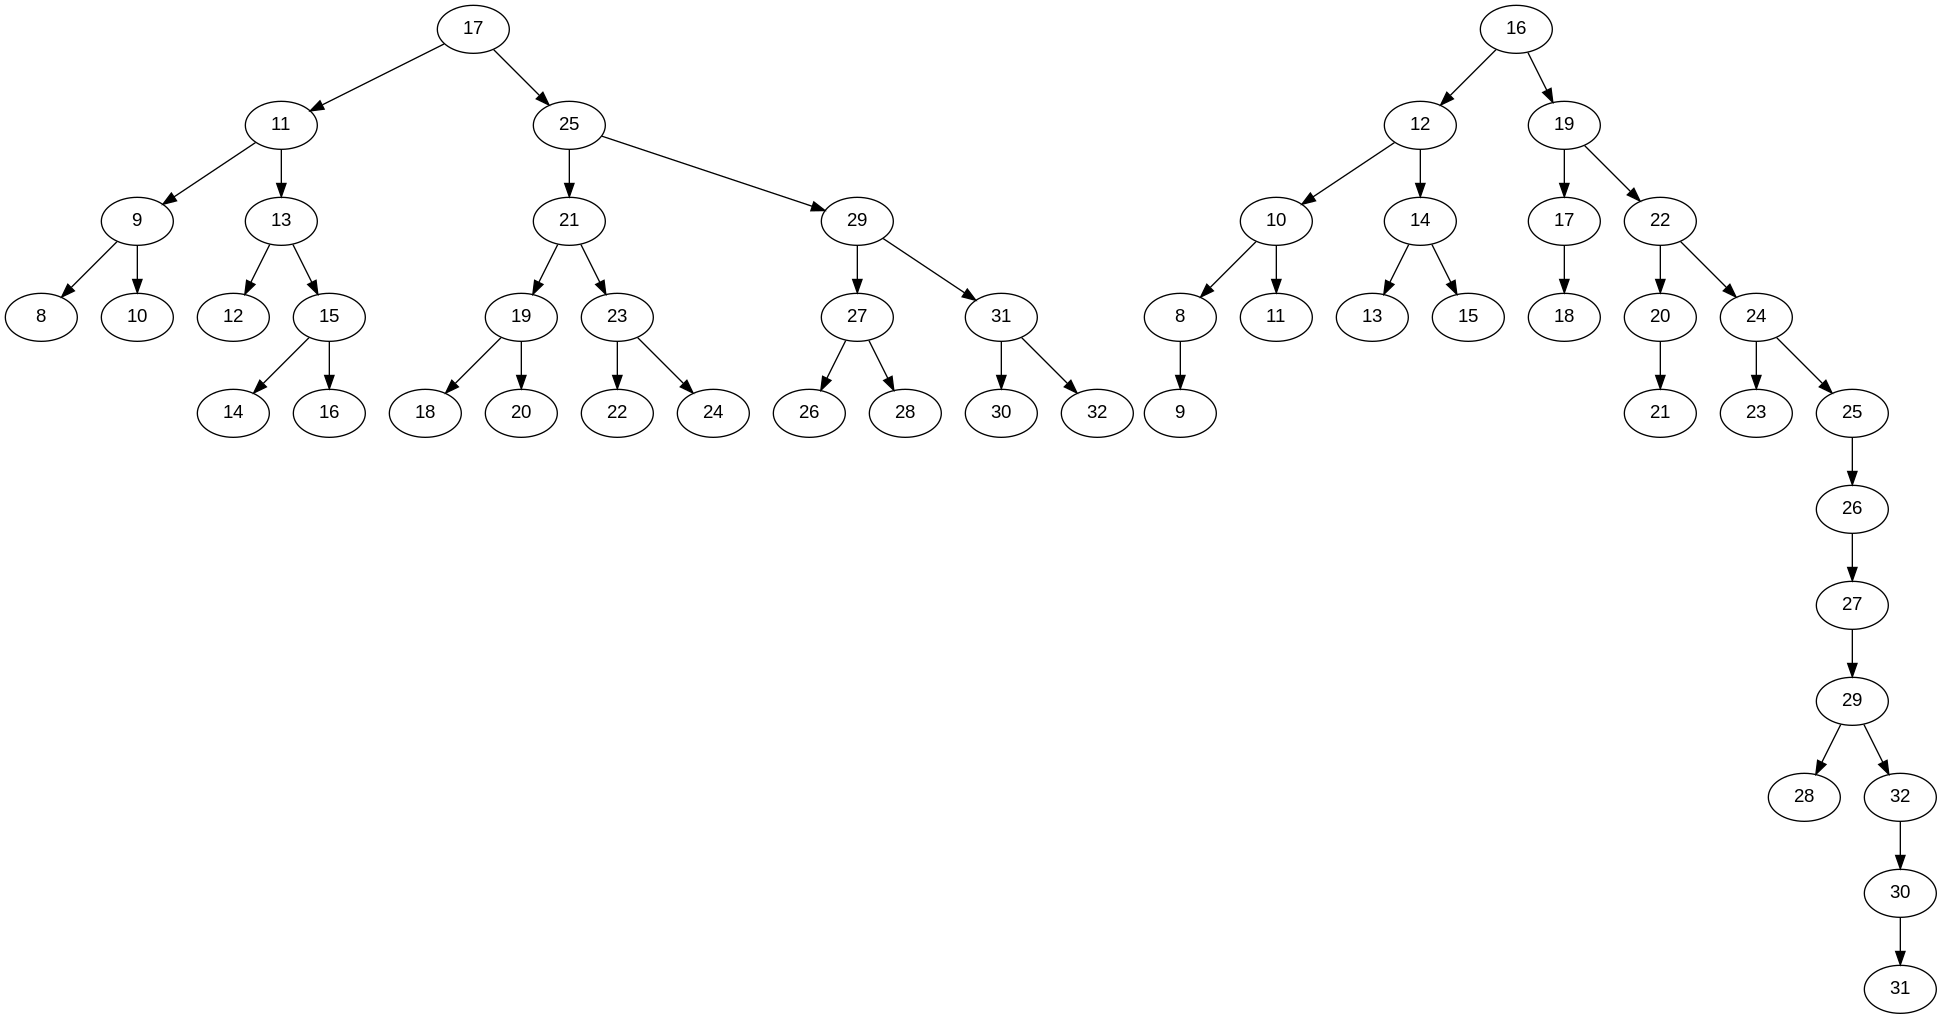
\includegraphics[height=2.0in]{../img/trees_v4.png}
  \caption{Balanced BST (used in experiments) vs. BST optimized exclusively for address share (not used), both based on the Route-Views.Oregon-ix.net IPv4 table}
\label{fig:trees-v4}
\end{figure}

We also contrast the performance of the linear vs. guided search schemes
benchmarked on IPv4 and IPv6 tables. We use two traffic pattern extremes:

\begin{enumerate}
\item random traffic, where most if not all IPv6 queries go to default route;
\item traffic correlated with the prefix length frequency distribution,
  using prefixes themselves as traffic.
\end{enumerate}

Finally, we observe the effect of the BF hyperparameters:
the bit vector size ($m$) -- or equivalently, the percentage of bits set -- 
and the count of hash functions ($k$) on the performance of the linear vs.
guided search schemes.

\begin{table}[]
\centering
\caption{Experiment Matrix} 
\label{tab:experiment-matrix}

\begin{tabular}{@{}lclcl@{}}
\toprule
traffic                 & \multicolumn{4}{c}{protocol}                        \\ \midrule
                        & \multicolumn{2}{c}{IPv4} & \multicolumn{2}{c}{IPv6} \\
random                  & \multicolumn{2}{c}{\checkmark}    & \multicolumn{2}{c}{\checkmark}    \\
by prefix address space & \multicolumn{2}{c}{\checkmark}    & \multicolumn{2}{c}{}     \\
by prefix frequency     & \multicolumn{2}{c}{\checkmark}    & \multicolumn{2}{c}{\checkmark}    \\ \bottomrule

\end{tabular}
\end{table}

\subsection{Discussion}

TBD...



\bibliographystyle{IEEEtran}
\bibliography{bibliography}
\end{document}
